% ==================== 2.3.2.6 锐钛矿 ====================
\jiegou{2.3.2.6}{锐钛矿结构（\texorpdfstring{TiO$_2$}{TiO2}）}

锐钛矿是 TiO$_2$ 的另一种常见晶型，属四方晶系，建模参数见表~\ref{tab:anatase}。
与金红石相比，锐钛矿晶胞为体心四方，$c$ 轴明显拉长。

\begin{table}[H]
  \centering
  \caption{锐钛矿（TiO$_2$）结构的建模参数}
  \label{tab:anatase}
  \begin{tabular}{ll}
    \toprule
    项目 & 参数 \\
    \midrule
    空间群 & $I\,4_1/a\,m\,d$（No.~141） \\
    晶格常数 & $a=b=3.784$\,\AA，$c=9.5146$\,\AA，$\alpha=\beta=\gamma=90^\circ$ \\
    原子坐标 & Ti：$(0,0,0)$（$4a$ 位）；O：$(0,0,0.208)$（$8e$ 位） \\
    化学式单元数 & $Z=4$ \\
    \bottomrule
  \end{tabular}
\end{table}

\begin{figure}[H]
  \centering
  \subcaptionbox{空间群与晶格常数设置}{%
    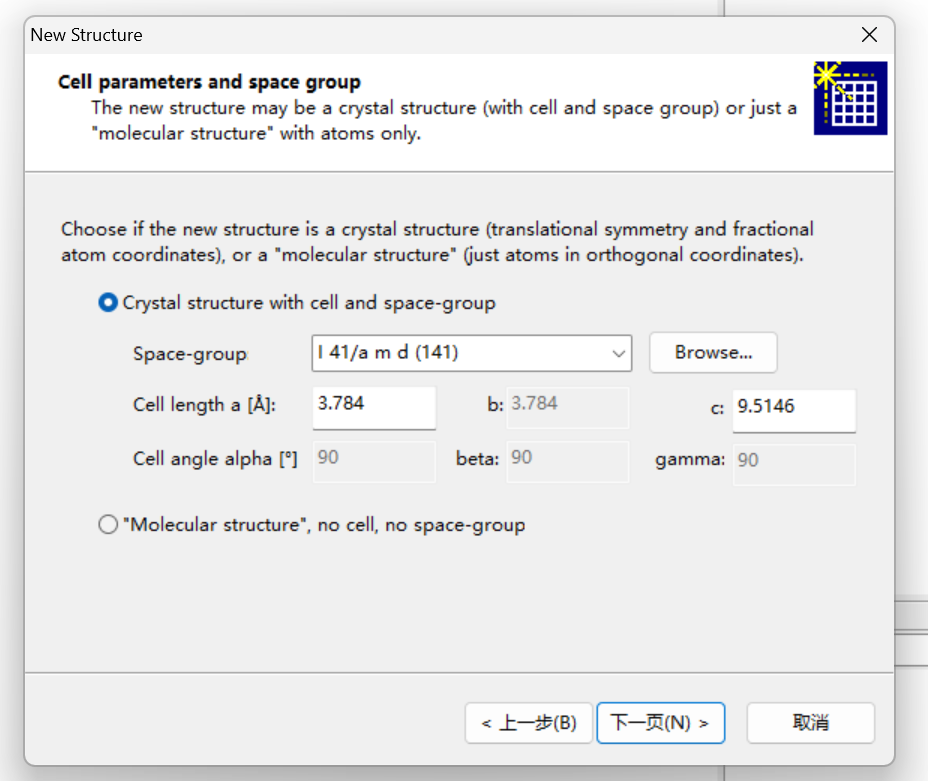
\includegraphics[width=0.44\textwidth]{assets/anatase/a.png}}
  \hfill
  \subcaptionbox{非对称单元原子（Ti、O）添加}{%
    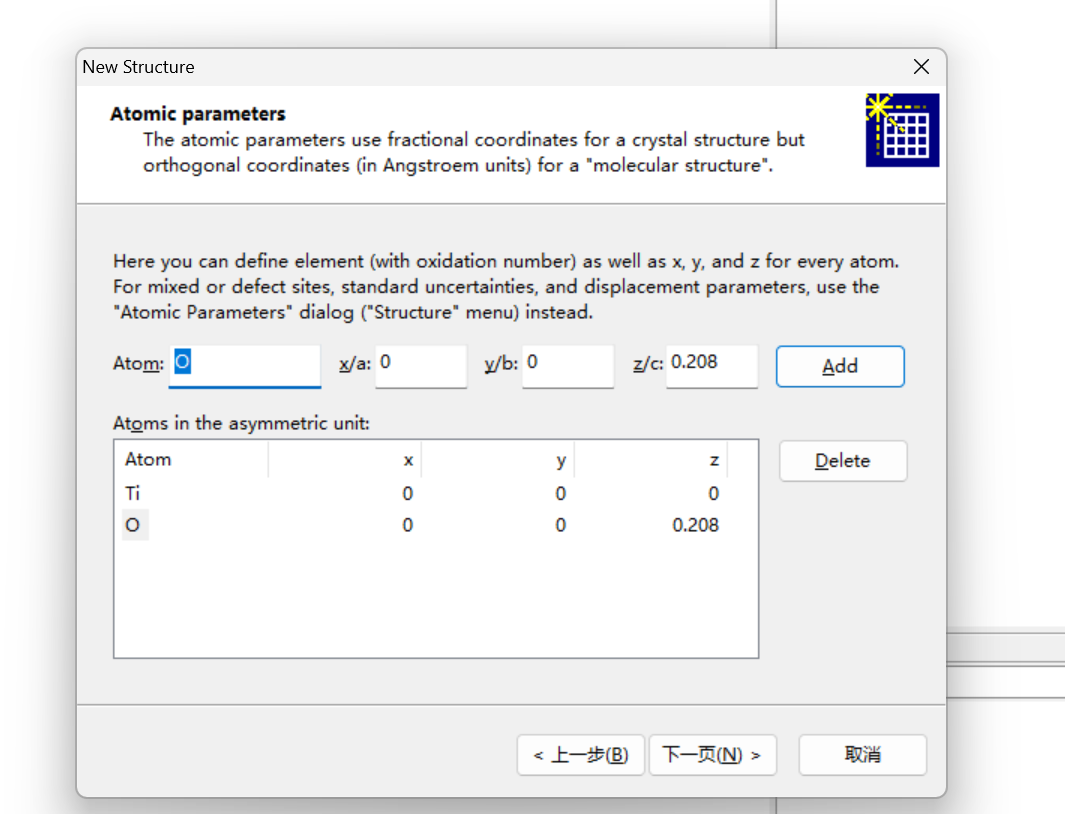
\includegraphics[width=0.44\textwidth]{assets/anatase/b.png}}
  \caption{锐钛矿（TiO$_2$）结构的参数设置}
  \label{fig:anatase-param}
\end{figure}

\begin{figure}[H]
  \centering
  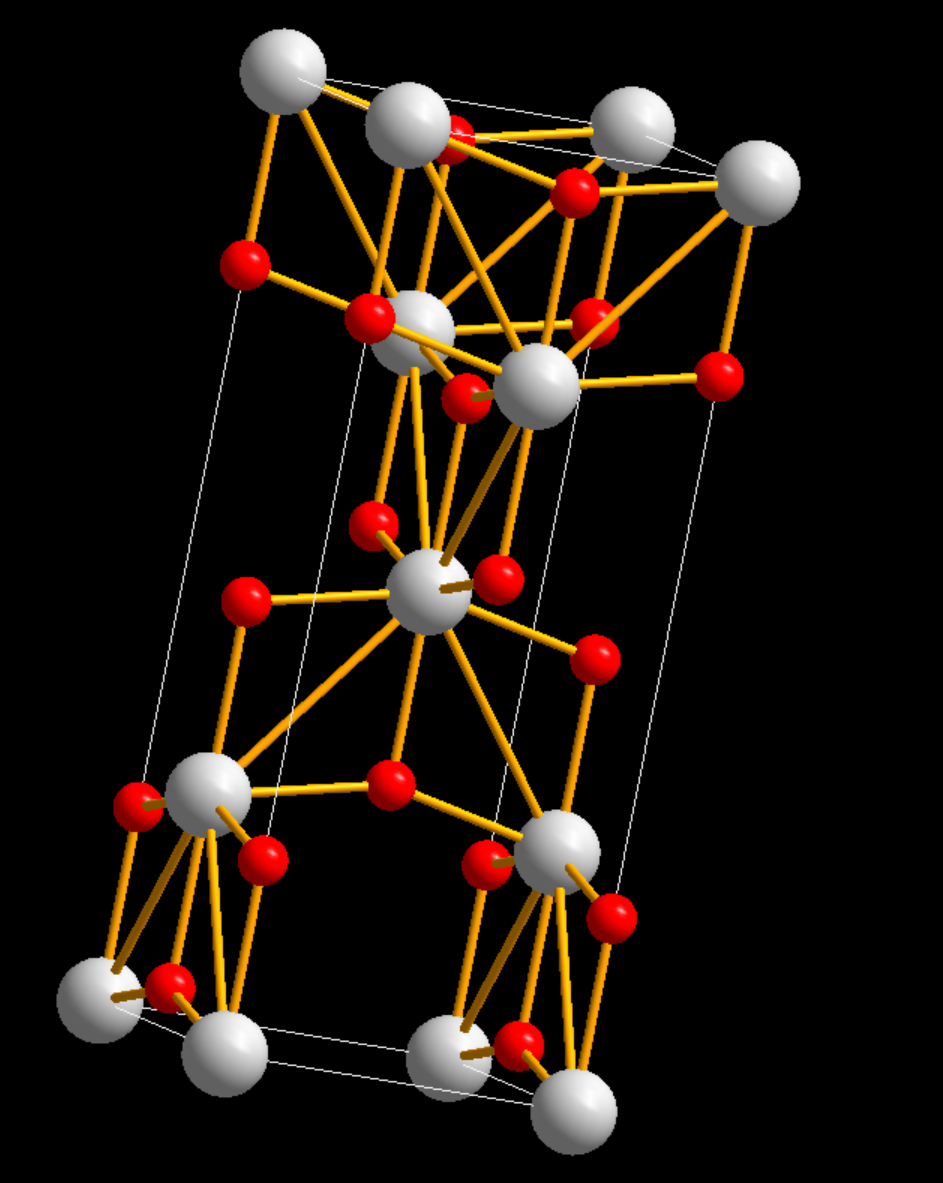
\includegraphics[width=0.5\textwidth]{assets/anatase/c.png}
  \caption{锐钛矿（TiO$_2$）结构的晶体结构模型}
  \label{fig:anatase-model}
\end{figure}

\begin{figure}[H]
  \centering
  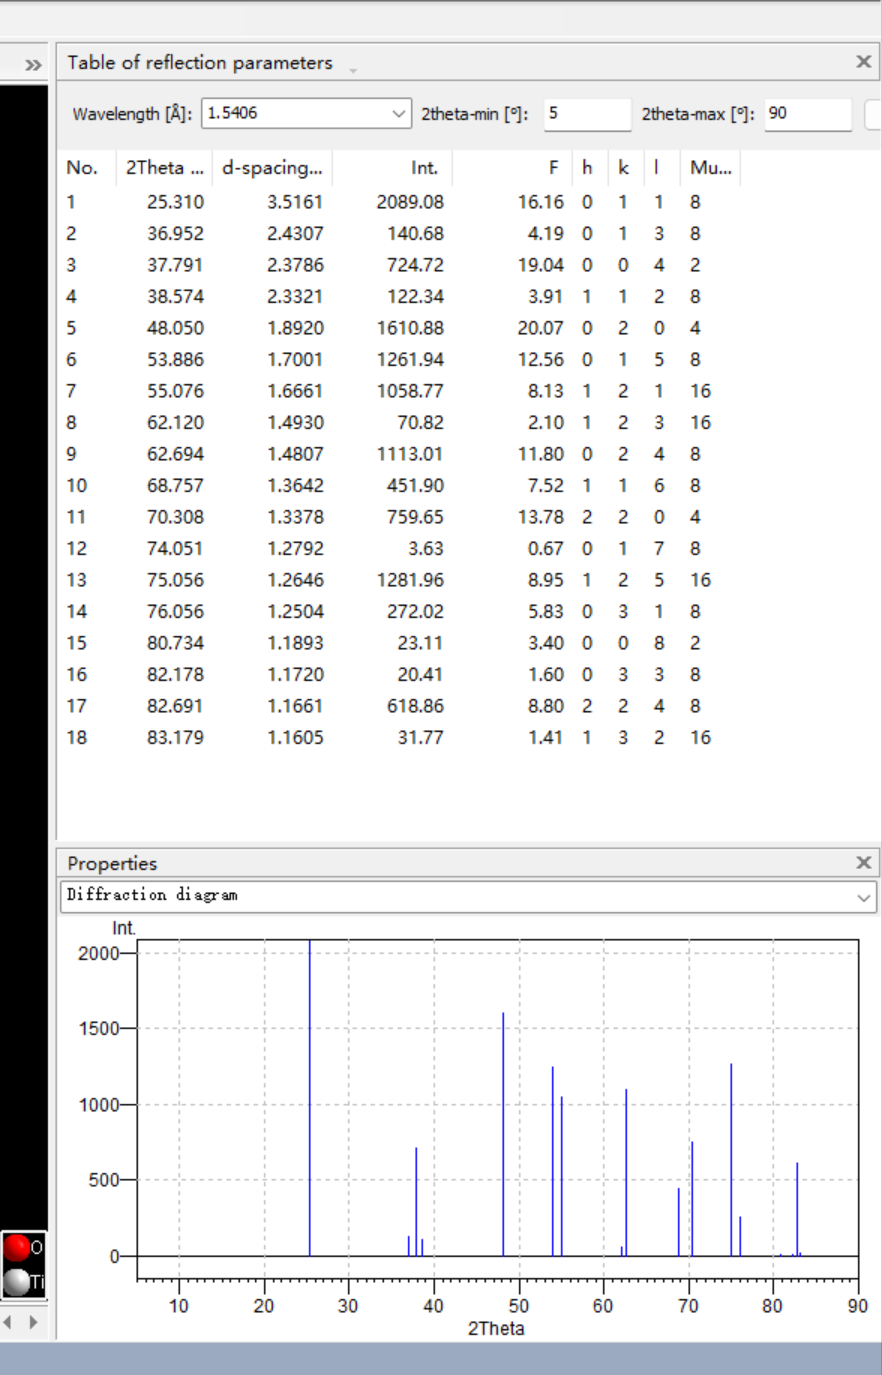
\includegraphics[width=0.4\textwidth]{assets/anatase/d.png}
  \caption{Diamond 模拟的锐钛矿（TiO$_2$）结构粉末衍射图}
  \label{fig:anatase-xrd}
\end{figure}

\begin{figure}[H]
  \centering
  \subcaptionbox{晶面视图}{%
    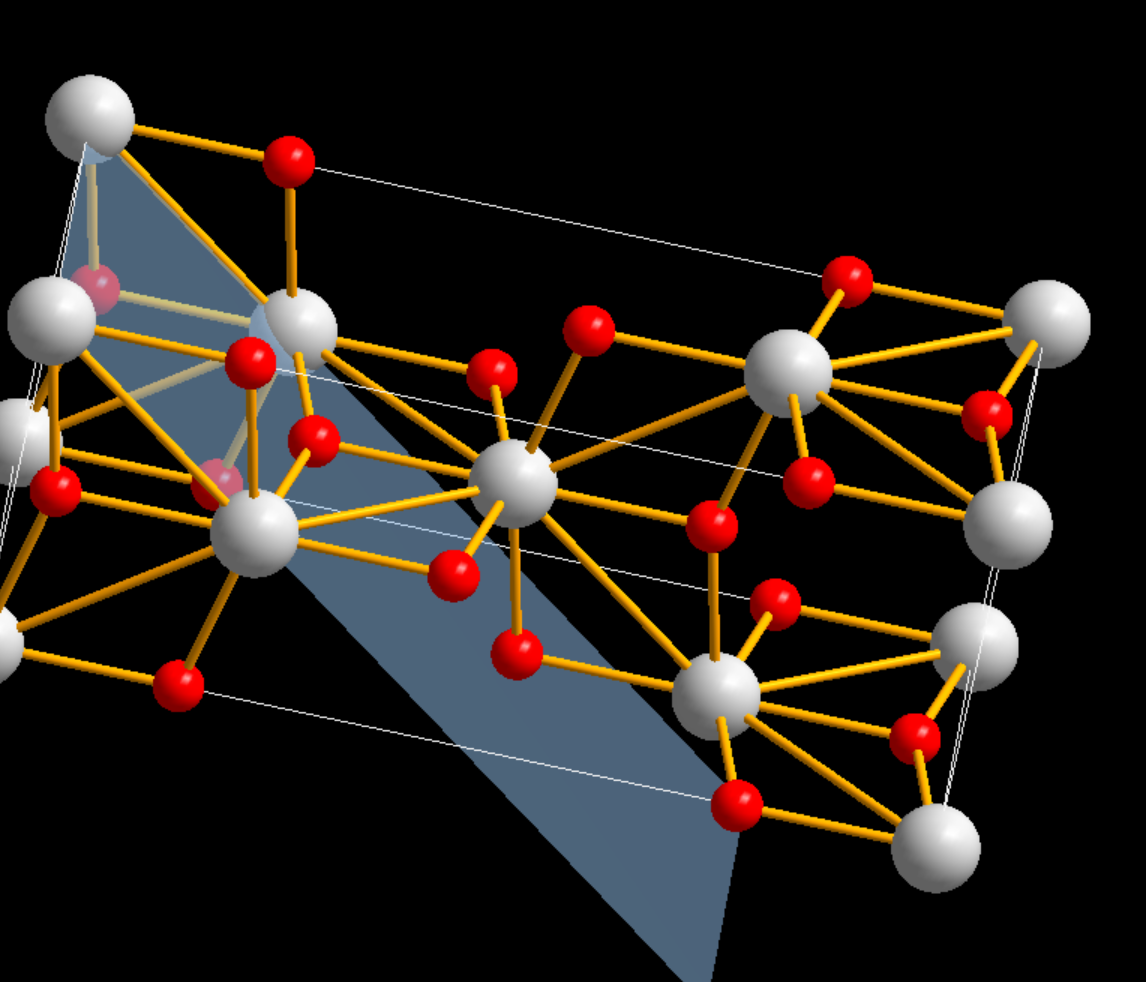
\includegraphics[width=0.44\textwidth]{assets/anatase/e.png}}
  \hfill
  \subcaptionbox{TiO$_6$ 配位八面体}{%
    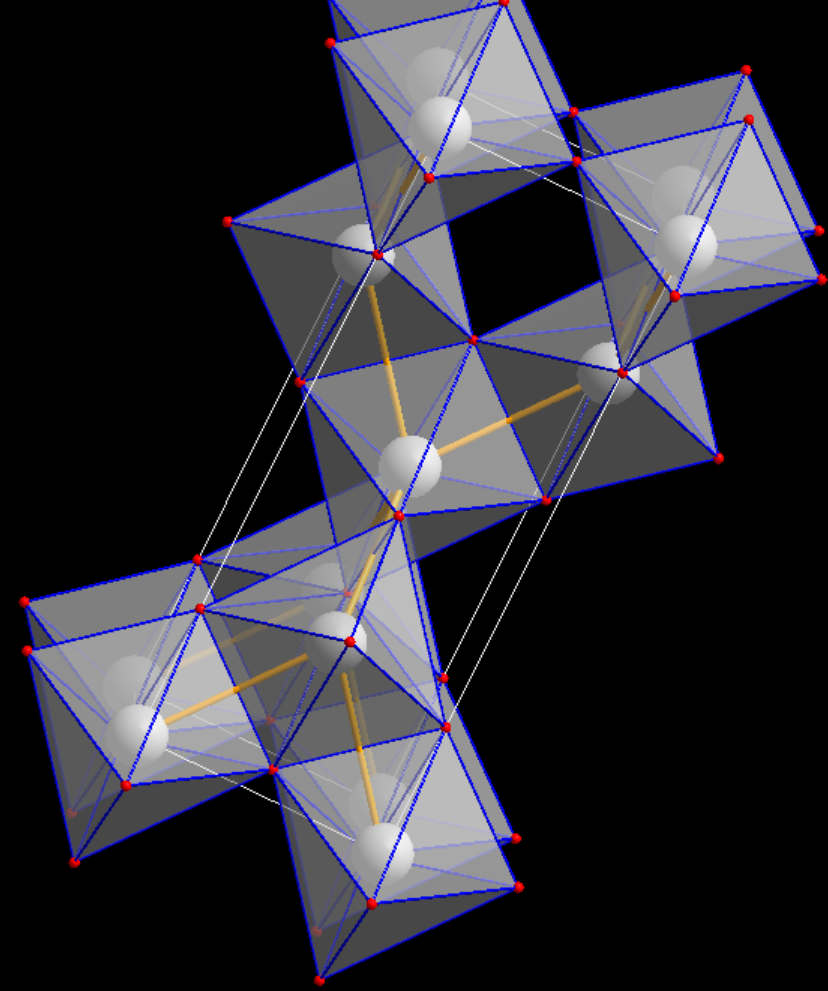
\includegraphics[width=0.28\textwidth]{assets/anatase/f.png}}
  \hfill
  \subcaptionbox{配位多面体设置}{%
    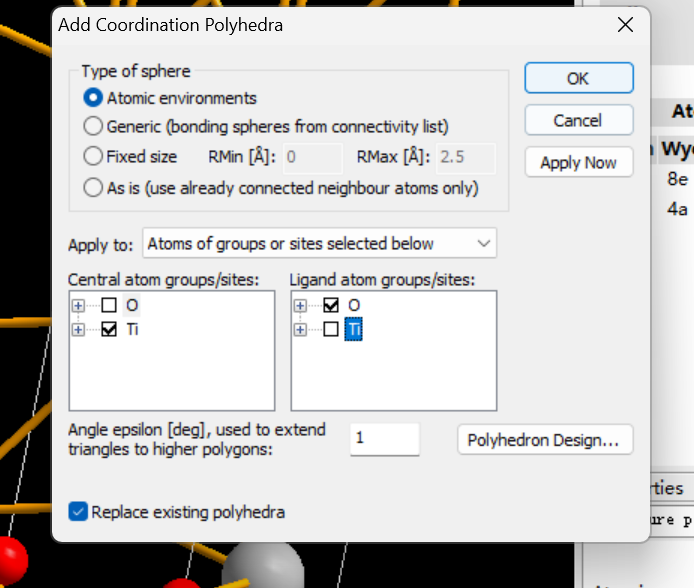
\includegraphics[width=0.24\textwidth]{assets/anatase/f1.png}}
  \caption{锐钛矿（TiO$_2$）结构的晶面与配位八面体}
  \label{fig:anatase-plane}
\end{figure}

\textbf{结构特征。}锐钛矿中 Ti$^{4+}$ 同样位于 TiO$_6$ 八面体中心，但八面体的连接
方式与金红石不同。

\begin{enumerate}[label=（\arabic*）]
  \item \textbf{TiO$_6$ 八面体}：由模型参数计算，沿 $c$ 轴方向的 2 个顶点 Ti--O 键长为
    $0.208\,c\approx1.98$\,\AA，赤道方向的 4 个 Ti--O 键长约为 $1.93$\,\AA
    （$=\sqrt{(a/2)^2+[(1/4-0.208)c]^2}$），八面体略有畸变。每个 O$^{2-}$ 与 3 个
    Ti$^{4+}$ 配位，其中 1 个键略长、2 个略短。
  \item \textbf{八面体的连接方式}：TiO$_6$ 八面体之间全部通过共边连接，形成沿
    $\langle100\rangle$、$\langle010\rangle$ 方向延伸的锯齿状链（图~\ref{fig:anatase-plane}(b)）。
    与金红石（共棱成链、链间共角）相比，锐钛矿的骨架更加开放，密度更低，晶胞中空位
    更大，这是锐钛矿 TiO$_2$ 在光催化等领域表现出特殊活性的结构原因之一。
  \item \textbf{空间群}：$I\,4_1/a\,m\,d$ 中 $I$ 为体心点阵，$4_1$ 螺旋轴沿 [001]，
    $a$ 滑移面、镜面 $m$ 与 $d$ 金刚石滑移面位于相应的特征方向。
\end{enumerate}

金红石与锐钛矿是 TiO$_2$ 最常见的两种晶型，二者的共同点是 TiO$_6$ 八面体配位，区别
在于八面体的连接方式，体现出``配位多面体—连接方式—晶体结构''的描述思路。
